\pagebreak

\section{Introduction to Information Theory}

Information theory is the study of communication over channels.
What is a channel?  Some examples of a channel are:
\begin{frml}
	Voice &\rightarrow Ears \\
	Eye &\rightarrow Brain \\
	DNA &\rightarrow DNA \\
	Antenna\;\; on\;\; Earth &\rightarrow Mars \;Rover \\
	Phone &\rightarrow Another Phone \\
\end{frml}
where the \textit{medium} of the channel is some physical system that the communication
is being transmitted over, e.g. in the case of Voice $\rightarrow $ 
Ears the medium is \textit{air}.

\begin{defn}{Fundamental Problem in Information Theory}{}
The \textbf{fundamental problem} in information theory is reliable communication 
over an unreliable channel.

\medskip
An \textbf{unreliable channel} is one where the \textit{received signal} is not equal
to the \textit{transmitted signal}, i.e.
\begin{frml}
	\text{Received Signal} \approx \text{Transmitted Signal} + \text{Noise}
\end{frml}
\end{defn}

There are two predominant soltuions that address this problem of unreliable channels.
The first option is a \textit{physical solution}, which attempts to address the physical
limitations of the medium to reduce the noise. Alternatively, there are \textit{system
solutions}, which accept the physical limitations of the channel, and attempt to
transform the overall system into a reliable one using \textit{encodings and decodings}.

Information theory is all about \textit{system solutions}. System solutions 
take the form of the pipeline below:

\begin{figure}[h!]
	\centering
\begin{tikzpicture}
[
encdecnode/.style={rectangle, draw=green!50!black, fill=green!5, very thick, minimum size=10mm, inner sep=10},
channelnode/.style={rectangle, draw=red!50!black, fill=red!5, very thick, minimum size=10mm, inner sep=10},
every node/.style={outer sep=7}
]
%Nodes
\node[]		(1) {$s$ };
\node[]		(1t) [below=.0cm of 1] {Source Message};
\node[encdecnode]        (2)       [right=of 1] {Encoder};
\node[]		(2t) [below=.7cm of 2] {Adds Redundancy};
\node[]        (3)       [right=of 2] {$t$};
\node[]		(3t) [below=.1cm of 3] {Coded Transmission};
\node[channelnode]        (4)       [right=of 3] {Channel};
\node[]		(4t) [below=.7cm of 4] {Adds Noise $n$};
\node[]        (5)       [right=of 4] {$r$};
\node[]		(5t) [below=.1cm of 5] {Received Transmission};
\node[encdecnode]        (6)       [right=of 5] {Decoder};
\node[]		(6t) [below=.7cm of 6] {Try to Infer $s$ and $n$};
\node[]        (7)       [right=of 6] {$\hat{s}$};
\node[]		(7t) [below=.1cm of 7] {Decoded message};

%Lines
\draw[->] (1.east) -- (2.west);
\draw[->] (2.east) -- (3.west);
\draw[->] (2t.north) -- (2.south);
\draw[->] (3.east) -- (4.west);
\draw[->] (4.east) -- (5.west);
\draw[->] (4t.north) -- (4.south);
\draw[->] (5.east) -- (6.west);
\draw[->] (6.east) -- (7.west);
\draw[->] (6t.north) -- (6.south);
%\draw[->] (uppercircle.south) -- (maintopic.north);
%\draw[->] (maintopic.east) -- (rightsquare.west);
%\draw[->] (rightsquare.south) .. controls +(down:7mm) and +(right:7mm) .. (lowercircle.east);
\end{tikzpicture}
\end{figure}

In this framework, the \textit{Encoder} and \textit{Decoder} are the focus of
system solutions.

\subsection{The Binary Symmetric Channel and Disk Drives}

To examine this in more detail, let's imagine an imaginary, toy, channel.
This channel is called the \textit{Binary Symmetric Channel}.

\begin{defn}{Binary Symmetric Channel}{}
	A \textbf{Binary Symmetric Channel}, with input $x$ and output $y$, follows
	the distribution
	\begin{frml}
		&P(y = 0 | x = 0) = 1 - f \\
		&P(y = 0 | x = 1) = f \\
		&P(y = 1 | x = 1) = 1 - f \\
		&P(y = 1 | x = 0) = f \\
	\end{frml}
i.e. with probability $f$, a bit of the input $x$ will be flipped. A diagram of
this channel might look like:
	\medskip
	\begin{center}
\begin{tikzpicture}
	\node[] (in) at (0,1) {Input $x$};
	\node[] (on) at (4,1) {Output $y$};
	\node[] (fn) at (2.1,1.3) {$f$};
	\node[] (tl) at (1,2) {0};
	\node[] (bl) [below=of tl] {1};
	\node[] (tr) [right=of tl] {0};
	\node[] (br) [right=of bl] {1};

	\path[->] (tl) edge node[midway, above] {$1 - f$} (tr);
	\path[->] (bl) edge node[midway, below] {$1 - f$} (br);
	\path[->] (tl) edge node[sloped, below] {} (br);
	\path[->] (bl) edge node[sloped, above] {} (tr);
\end{tikzpicture}
\end{center}
\end{defn}

Suppose we have a disk drive which follows the behavior of a binary
symmetric channel with $f = 0.1$. 

If a file of $N=10,000$ bits is stored
and then read from this disk drive, roughly how many bits will be flipped?
The answer can be modeled as a binomial distribution. 
The event of each bit being flipped or not is an independent event.
Binomial distributions have mean $Np$ and variance $Npq$, 
where in this problem $p = f$ and $q = 1 - f$.
Thus the answer is:
\begin{frml}
	\text{\# of bits flipped } = 1000 \pm 30
\end{frml}
This is \textit{not a good disk drive}. We're flipping far too many bits, here.

Instead lets ask the question: How small does $f$ need to be in order to have
a disk drive that is reliable?
Imagine that 1GB of data is written every day,
for 5 years. This results in the number of bits being sent through this
channel to be
\begin{frml}
	\text{\# of bits passed} = 5 \times 365 \times 8 \times 10^9 \approx 10^{13}
\end{frml}
In order to guarantee a 1\% chance that a any file has a single bit flipped in
5 years, then we need $f\approx10^{-15}$.
The mean and standard deviation of the number of bits flipped is modeled by
the distribution:
\begin{frml}
	\text{Mean: }&Np = 10^{13}\times10^{-15} = 10^{-2} = 0.01 \\
	\text{Std: }&\sqrt{Npq} =  \sqrt{10^{13}\times10^{-15}\times(1 - 10^{-15})} \approx 0.1
\end{frml}
Thus, with $f = 10^{-15}$ the number of bits that will flip in 5 years of use is
$0.01 \pm 0.1$

\subsection{Repitition Encoding and Decoding}

One natural way to address this problem is to add redundancy to our encoding,
increasing the chances that we can recover a source from noise.
The simplest method for adding redundancy is called the \textit{repitition code}.

\begin{defn}{Repition Code}{}
A repitition code $R_k$ encodes source $s$ by repeating each bit of $s$ $k$-times
in transmission $t$.	

\medskip
For example, $R_3$ follows the following protocol:

\medskip
\begin{center}
\begin{tikzpicture}
	\node[] (r) at (1.5,2) {$R_3$};
	\node[] (p1) at (0,1.35) {};
	\node[] (p2) at (2.8,1.35) {};
	\node[] (in1) at (0.5,1) {1};
	\node[] (ins) at (2.2,1.6) {$t$};
	\node[] (int) at (0.5,1.6) {$s$};
	\node[] (out1) [right=of in1] {111};
	\node[] (in0) [below=0.3cm of in1]  {0};
	\node[] (out0) [right=of in0] {000};

	\path[->] (in1) edge node[midway, above] {} (out1);
	\path[->] (in0) edge node[midway, above] {} (out0);
	\path[-] (p1) edge node[midway, above] {} (p2);
\end{tikzpicture}
\end{center}

\end{defn}

Following the $R_3$ protocol, suppose we have the following transmission:
\begin{frml}
	s &= 0 1 1 0 1 \\
	t &= 000\; 111\; 111\; 000\; 111 \\
	n &= 000\; 100\; 000\; 101\; 000 \\
	r &= 000\; 011\; 111\; 101\; 111 \\
\end{frml}

How should we decode this file? A trivial solution is to take the majority
vote of each repetition. This would recover the solution, $\hat s$ as:
\begin{frml}
	\hat s = 0 1 1 1 1
\end{frml}
Let's look at why this is the correct decoder.

\subsubsection{Decoding is Inference}

\textit{Decoding is inference}: We want to 
\textit{infer} the correct source given the recieved signal.
To do this, we need to rely on \textit{inverse probability}. 
Inverse probability relies on two fundamental rules of probability:
\begin{defn}{Fundamental Rules of Probability}{}
	There are two fundamental rules in probability.

	\medskip
The \textbf{Product Rule} states that the probability of any two random variables
is equal to the probability of one random variable times the probability of the 
other random variable given the first.
\begin{frml}
	\text{Product Rule: } P(s, r) &= P(s) P(r|s) \\
								  &= P(r) P(s|r) \\
\end{frml}

The \textbf{Sum Rule} states how to retreive a marginal probability by the
sum of all the joint variables.
\begin{frml}
	\text{Sum Rule: } P(r) &= \sum_s P(s, r)
\end{frml}
\end{defn}

Now, if we reveive an $r$, then what we want is to infer $P(s | r)$, which is
called the \textit{Posterior probability of $s$}. We can use the product rule 
combined with the sum rule to
obtain this value.

\begin{defn}{Posterior Probability of $s$ }{}
	Given a recieved signal $r$, the \textbf{posterior of $s$ } is defined as:
\begin{frml}
	P(s | r) &= \frac{P(s)P(s, r)}{P(r)} 
			 = \frac{P(s)P(s, r)}{\sum_{s'} P(r,s')}
\end{frml}
Here, we call
\begin{itemize}
	\item $P(s)$ the \textit{prior} of $s$ 
	\item $P(r,s)$ the \textit{likelihood} of $s$
\end{itemize}
\end{defn}

For example, if we are using $R_3$ over a binary symmetric channel, 
and we recieve $r = 011$, then
\begin{frml}
	P(r | s = 0) &= (1 - f) \times f \times f &= (1-f)^1 f^2\\
	P(r | s = 1) &= f \times (1 - f) \times (1 - f) &= f^1 (1 - f)^2\\
\end{frml}

If we assume that, in general,  
\begin{frml}
	P(s=0) = \frac{1}{2}, \text{ and }
	P(s=1) = \frac{1}{2}
\end{frml}
then  we can obtain the posterior distribution:
\begin{frml}
	P(s=1 | r = 011) = \frac{f(1 - f)^2\frac{1}{2}}{(1 - f)f^2\frac{1}{2} + f(1-f)^2\frac{1}{2}}
	= 1 - f
\end{frml}

Thus, given our decoding scheme for $R_3$, we can say that $P(s = 1 | r = 011) = 1 - f$, which
is $90\%$ if $f = 0.1$. So, this is a reasonable decoding scheme.
Since $P(s=1|r) > P(s=0|r)$, then $\hat s = 1$ is the best guess.

\subsubsection{Rate and Error}

Suppose we are sending a message $s$ over  Binary Symmetric Channel with flip
probability of $f$, using $R_3$ encoding and Majority Vote Decoding. 
What is the probability
that a \textit{single} bit is flipped? There are \textit{two} outcomes which must
be considered here. The probability that 3 bits in a single chunk were flipped
and the probability that 2 bits in a single chunk were flipped, i.e.
\begin{frml}
	\text{For one bit: } P(\hat s \neq s) = f^3 + 3f^2(1 - f) \approx 3f^2 - 2f^3
\end{frml}
where the $3$ comes from the $3$ different ways to \textit{choose} which bits are
flipped. This term is dominated by the $3f^2$. What have we achieved with this
encoding scheme? 
We have decreased the \textbf{rate} of our transmitting from $1$ to $1/3$. In 
doing so, we have decreased the probability of bit error from $f$ to $3f^2$.
Thus, by using 3 bits for every bit, we have achieved a \textbf{bit error rate} 
of $3f^2$.

Let's return, briefly, to the disk drive problem we were considering earlier.
Assuming again that our $f=0.1$, how many repititions do we need (i.e. what $k$ of
$R_k$) to get the bit error rate below $10^{-15}$?

It turns out that in order to achieve our desired
reliability of $10^{-15}$ 
$k$ will need to be approximately $61$. This is rather terrible, as it means
that we will need 61 \textit{individual} gigabyte disk drives in order to ensure
the reliability of a single GB disk drive.
We can do much better than this!

\subsection{The 7,4 Hamming Code}

The 7,4 Hamming Code gives us a much more efficient encoding, in terms of rate
vs bit-error rate, than repitition encoding. It utilizes \textit{parity codes}, 
which represent the parity between bits in a message.

\begin{defn}{The 7,4 Hamming Code}{}
	The 7,4 Hamming Code takes in source bits $s_1, s_2, s_3, s_4$ and outputs
	transmission $t = [ s_1, s_2, s_3, s_4, t_5, t_6, t_7 ]$. Thus for every
	4 source bits, we output 7, giving us a rate of 4/7.

\medskip
	The \textit{parity} bits, $t_5, t_6, t_7$ are determined by the parity of
	subsets of $s$. The subsets of $s$ which correspond to each $t$ are 
	shown in the diagram below.
\medskip
\begin{center}
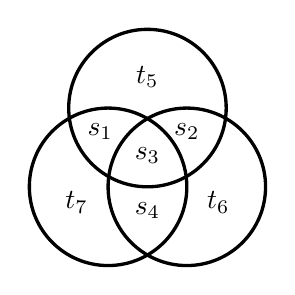
\begin{tikzpicture}
[
hamcircle/.style={circle, draw=black, very thick, minimum size=20mm, inner sep=10}
]
%Nodes
\node[hamcircle] at(5,4)		(t) {};
\node[hamcircle] at(5.5,5)		(l) {};
\node[hamcircle] at(6,4)		(r) {};
\node[]		(s1) at(4.9,4.7) {$s_1$};
\node[]		(s2) at(6.0,4.7) {$s_2$};
\node[]		(s3) at(5.5,4.4) {$s_3$};
\node[]		(s4) at(5.5,3.7) {$s_4$};
\node[]		(t5) at(5.5,5.4) {$t_5$};
\node[]		(t6) at(6.4,3.8) {$t_6$};
\node[]		(t7) at(4.6,3.8) {$t_7$};

\end{tikzpicture}
\end{center}

\end{defn}

Let's look at a couple examples of how a source $s$ is transmitted as $t$.
\begin{center}
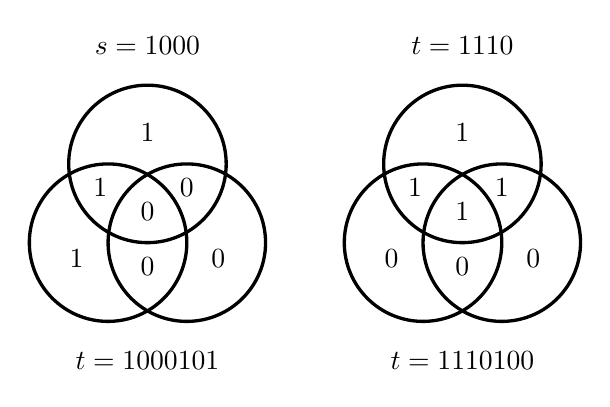
\begin{tikzpicture}
[
hamcircle/.style={circle, draw=black, very thick, minimum size=20mm, inner sep=10}
]
%Nodes
\node[]		(s) at(3.5,6.5) {$s = 1000$};
\node[]		(t1) at(7.5,6.5) {$t = 1110$};
\node[hamcircle] at(3,4)		(t) {};
\node[hamcircle] at(3.5,5)		(l) {};
\node[hamcircle] at(4,4)		(r) {};
\node[]		(s1) at(2.9,4.7) {$1$};
\node[]		(s2) at(4.0,4.7) {$0$};
\node[]		(s3) at(3.5,4.4) {$0$};
\node[]		(s4) at(3.5,3.7) {$0$};
\node[]		(t5) at(3.5,5.4) {$1$};
\node[]		(t6) at(4.4,3.8) {$0$};
\node[]		(t7) at(2.6,3.8) {$1$};
\node[]		(t1) at(3.5,2.5) {$t = 1000101$};
\node[]		(t1) at(7.5,2.5) {$t = 1110100$};

\node[hamcircle] at(7,4)		(t) {};
\node[hamcircle] at(7.5,5)		(l) {};
\node[hamcircle] at(8,4)		(r) {};
\node[]		(s21) at(6.9,4.7) {$1$};
\node[]		(s22) at(8.0,4.7) {$1$};
\node[]		(s23) at(7.5,4.4) {$1$};
\node[]		(s24) at(7.5,3.7) {$0$};
\node[]		(t25) at(7.5,5.4) {$1$};
\node[]		(t26) at(8.4,3.8) {$0$};
\node[]		(t27) at(6.6,3.8) {$0$};

\end{tikzpicture}
\end{center}

How does our decoder work, for this encoding?
Recall that the general idea is:
\begin{frml}
	P(s|r) = \frac{P(r|s)P(s)}{P(r)}
\end{frml}

where our likelihood $P(r|s)$ favors $s$ that require fewer bit flips to achieve $r$.
Let's take a look at what $r$ looks like:

\begin{center}
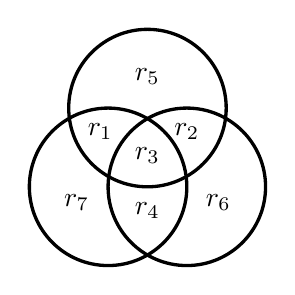
\begin{tikzpicture}
[
hamcircle/.style={circle, draw=black, very thick, minimum size=20mm, inner sep=10}
]
%Nodes
\node[hamcircle] at(5,4)		(t) {};
\node[hamcircle] at(5.5,5)		(l) {};
\node[hamcircle] at(6,4)		(r) {};
\node[]		(s1) at(4.9,4.7) {$r_1$};
\node[]		(s2) at(6.0,4.7) {$r_2$};
\node[]		(s3) at(5.5,4.4) {$r_3$};
\node[]		(s4) at(5.5,3.7) {$r_4$};
\node[]		(t5) at(5.5,5.4) {$r_5$};
\node[]		(t6) at(6.4,3.8) {$r_6$};
\node[]		(t7) at(4.6,3.8) {$r_7$};
\end{tikzpicture}
\end{center}

Let's again imagine that we sent the source 
$s = 1000$ with transmission $t = 1000101$.

Assume that $r_2$ is flipped, resulting in $r = 1100101$,
resulting in the following diagram

\begin{center}
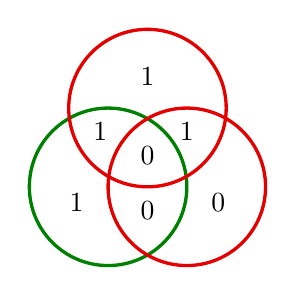
\begin{tikzpicture}
[
happyhamcircle/.style={circle, draw=green!50!black, very thick, minimum size=20mm, inner sep=10},
badhamcircle/.style={circle, draw=red!90!black, very thick, minimum size=20mm, inner sep=10}
]
%Nodes
\node[happyhamcircle] at(5,4)		(t) {};
\node[badhamcircle] at(5.5,5)		(l) {};
\node[badhamcircle] at(6,4)		(r) {};
\node[]		(s1) at(4.9,4.7) {$1$};
\node[]		(s2) at(6.0,4.7) {$1$};
\node[]		(s3) at(5.5,4.4) {$0$};
\node[]		(s4) at(5.5,3.7) {$0$};
\node[]		(t5) at(5.5,5.4) {$1$};
\node[]		(t6) at(6.4,3.8) {$0$};
\node[]		(t7) at(4.6,3.8) {$1$};
\end{tikzpicture}
\end{center}

Here we can see that two parity bits are off, and one is correct, due to $r_2$
being flipped. So, our rule is going to be to: find the bit that is inside
each sad circle, and outside each happy circle, and identify it as the bit
that was flipped. Thus, our guess for $t = 1000101$, and our guess for the
message is $\hat s = 1000$.

It is the case that  \textbf{for any single flip}, this decoding method will always
detect the correct flip. However, if more than one flip occurs, then we will not
guess the correct s.
Using this code, the probability of a block error is about $21f^2$ and the probability
of a bit error is $9f^2$. Thus, we can see that we actually have a higher bit error
rate than the $R_3$ encoding, but we have a much \textit{larger} rate.

So we can see that we're playing this tradeoff game between the \textit{rate} of an 
encoding, and the \textit{bit error rate}. How good can we actually do on this?
The answer to this is exaclty Shannon's Theorem.

\subsubsection{Shannon's Theorem, informally}

Shannons Theorem states that there is \textit{always} an encoding with
a \textit{non-zero} rate which achieves 0 bit-error rate. The rate of this
\textit{optimal} encoding is called the capacity $C$.

For example, Shannons theorem states that the capacity of a Binary Symmetric
Channel with flip probability $f$ is
\begin{frml}
	C_{BSC(f)} &= 1 - H_2(f) \\
	H_2(f) &= f \log \frac{1}{f} + (1 - f)\log \frac{1}{1-f}
\end{frml}

This is rather remarkable. Recall that our $R_3$ encoding told us that, with
$f=0.1,$ in order
to get a bit-error rate of $10^{-15}$ for our disk drives, we actually needed
a total of $61$ disk drives. However, shannons theorem tells us that there is
an encoding for which \textit{we only need $2$ disk drives!}
